%(BEGIN_QUESTION)
% Copyright 2006, Tony R. Kuphaldt, released under the Creative Commons Attribution License (v 1.0)
% This means you may do almost anything with this work of mine, so long as you give me proper credit

Når lastceller brukes til nivåmåling i tanker, må visse forholdsregler tas for å sikre nøyaktige målinger:

$$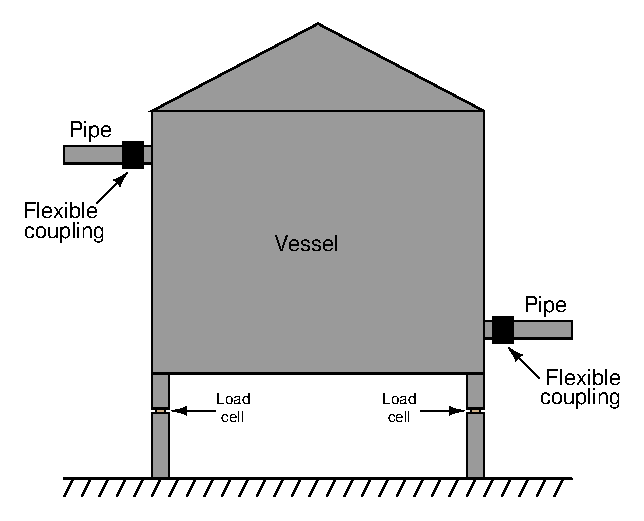
\includegraphics[width=15.5cm]{i00326x01.eps}$$

En viktig forholdsregel er å montere fleksible koblinger på alle rør inn til og ut fra tanken. Stive rør vil gi målefeil. Forklar hvorfor.

\vskip 10pt

Anta at denne (vertikale) sylindriske lagringstanken har en diameter på 10 fot, høyde 8 fot fra bunnen av tanken til foten av det koniske taket (11 fot fra bunnen av tanken til mønet), er laget helt i bløtt stål og veier 12,933 pund når den er tom. Beregn væskenivået i tanken når målt totalvekt er 40,854 pund. Anta en væske med tetthet 60.5 pund per kubikkfot.

\vskip 20pt \vbox{\hrule \hbox{\strut \vrule{} {\bf Forslag til sokratisk diskusjon} \vrule} \hrule}

\begin{itemize}
\item{} Nevn noen praktiske anvendelser i industrien der vektbasert nivåmåling er å foretrekke fremfor andre teknologier.
\item{} En faktor som kan gi målefeil i systemer som dette, er \textit{vær}, i hvert fall for tanker utendørs. Nevn konkrete værforhold som kan skape problemer, og forklar hvordan disse vil vises i tankens nivåsignal.
\end{itemize}

\underbar{file i00326}
%(END_QUESTION)





%(BEGIN_ANSWER)

Væskenivå = 5 fot 10.5 tommer fra bunnen av tanken

%(END_ANSWER)





%(BEGIN_NOTES)

Eksterne rør må ikke få bære noen del av tankens vekt.

\vskip 10pt

Totalvekt $-$ taravekt = produktvekt

\vskip 10pt

40854 lb $-$ 12933 lb = 27921 lb

$$F = \gamma V$$

$$V = {F \over \gamma} = {27921 \hbox{ lb} \over 60.5 \hbox{ lb/ft}^3} = 461.5 \hbox{ ft}^3$$

$$V = Ah$$

$$h = {V \over A}$$

$$A = \pi r^2 = \pi 5^2 = 78.54 \hbox{ ft}^2$$

$$h = {V \over A} = {461.5 \hbox{ ft}^3 \over 78.54 \hbox{ ft}^2} = 5.876 \hbox{ ft} = 5 \hbox{ ft } 10.5 \hbox{ in}$$

\vskip 10pt

Tankmaterialet (bløtt stål) er overflødig informasjon, tatt med for å utfordre studenten til å vurdere om opplysninger er relevante for å løse en konkret oppgave.

%INDEX% Measurement, level: load cell

%(END_NOTES)
